\section{Motivating Example}\label{sec:motivating}

\begin{figure}[t]
    \centering
    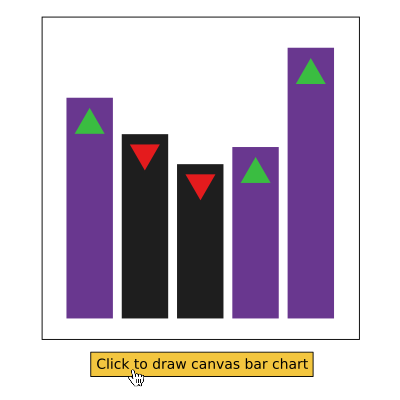
\includegraphics[trim={0.1cm 0.1cm 0.1cm 0.1cm},clip,width=0.58\textwidth,height=0.36\textheight]{testability/figures/motivating-example-new.png}
    \caption{An example canvas-based application. When the button is clicked, the plot is drawn dynamically (on the client side) using the canvas element.}
    \label{fig:motivating-example-1}
\end{figure}


Figure~\ref{fig:motivating-example-1} shows an example web application that uses canvas elements.
A bar chart is drawn in the canvas when the user clicks the button.
The corresponding JavaScript code is shown in Listing~\ref{lst:motivating-example-1}.
This example illustrates the dynamic nature of canvas-based web applications.
The data is plotted dynamically, on-the-fly, on the client side as opposed to the latency involved in sending the data to be plotted at a server that replies back with an image of the generated bar chart.
This dynamic nature makes canvas elements useful in interactive and high-performance visualizations and graphics.

Listing~\ref{lst:motivating-example-1} shows a snippet of how the setup and manipulation of canvas elements is done exclusively through the Canvas JavaScript API~\cite{w3c_canvas_standard}.
The canvas API provides functionality to draw lines, circles, rectangles, etc.
These can then be combined and dynamically added to the canvas element in order to draw more complex and interactive drawings.
Lines 6 to 11 show a snippet of how the canvas API is used to draw a rectangle on the chart.
A call is made to the \verb|fillRect()| function from the canvas API with parameters specifying the rectangle.
This allows dynamic creation of shapes on the canvas.

However, the HTML canvas element itself (Listing~\ref{lst:motivating-example-1}, lines 17-21)  remains empty throughout the entire usage of the application.
The execution of various canvas API functions does not change or update the contents of the canvas element tag.
\hl{This is because, as required by the official W3C standard~\mbox{\cite{w3c_canvas_standard}} of canvas elements, the canvas has no DOM representation. That is, the DOM subtree under a canvas node remains empty, and therefore its state remains unobservable. 
Instead, the canvas API functions are required to draw \mbox{\emph{directly}} to the raw monitor pixels buffer without the costly task of maintaining a DOM representation. This direct drawing allows canvas elements to achieve high-speed performance in order to enable dynamic and highly-interactive applications. }

Unfortunately, this DOM-free nature that enables the high-speed of canvas elements is also the reason why they are more difficult to test.
At any point during the execution of the application, the state of the canvas remains unobservable.
While one might conceptually think of gathering state information by tracking the call stack of the API calls, this would not be applicable to an exclusively visual API such as that of the canvas.
This is because the actual visual rendered canvas does not directly correspond to the calls made to its API.
For instance, calls could mistakenly visually override one another, or they might call the API with unintended arguments, resulting in a wrong visual result. 
A thousand canvas API calls (for example, draw the rectangle in the example, \emph{one point} at a time) can produce the same resulting visual state as one canvas call (a single call to \verb|fillRect|).
Consequently, we can see that it is difficult to assess what state is the canvas in at any given moment which makes it difficult to test canvas elements.

\hl{In this chapter, we propose an approach that makes canvas elements testable. That is, the goal is to 
provide developers with the fundamental capability of observing the canvas state and making assertions on it. However, the aim is not to provide a complete testing solution, but rather to enable the 
testing process itself, thereby improving testability. This approach visually analyzes the canvas screenshot, then creates a DOM tree representing the visual state of the canvas.
This makes it possible to test the canvas element using common DOM-testing techniques.
Finally, the developers would write their own tests, or could optionally use the automatically generated tests to check the visual objects of the canvas and their properties.}


\begin{lstlisting}[language={javascript},
float=tbp,
aboveskip=1.4em,
caption=JavaScript and HTML snippet of the canvas drawing in Figure~\ref{fig:motivating-example-1}., 
label={lst:motivating-example-1}]

function onButtonClick() {
	var canvas = document.getElementById("canvasBarChart
").getContext("2d");
	...
	canvas.beginPath();
	...
	// Example: this would draw one of the
	// rectangles in the bar chart.
	canvas.fillRect(leftCoordinate, topCoordinate,
					width, height);
	...
}


// The HTML portion of the app
<canvas id="canvasBarChart">
	// This tag remains empty throughout the usage of
	// the app, due to the lack of DOM representation
	// for canvas elements.
</canvas>

\end{lstlisting}